\chapter{Gra karciana Love Letter}
\label{cha:rozdz2}

W tym rozdziale opisuję kontekst oraz zasady gry Love Letter. Opisuję działanie każdej karty oraz przedstawiam główny cel gry - wygranie określonej ilości rund. Następnie przedstawiam problem i analizuję jego złożoność. Wszystkie załączone zdjęcia oraz instrukcja zaczerpnięte są z [\ref{bib:loveLetterGame}] oraz [\ref{bib:loveLetterWebsite}].

\begin{figure}[h]
	\centering
	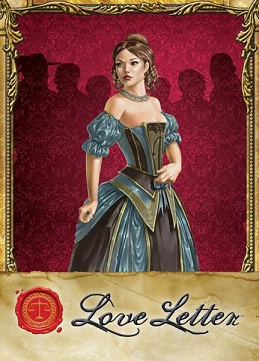
\includegraphics{Resources/ll_main_image.png}
	\caption{Love Letter - okładka} 
	\label{fig:llMainImage}
\end{figure}

\section{Opis zasad gry}
\label{sec:opisGry}
W trakcie gry wcielamy się w rolę jednego z adoratorów księżniczki starającego się o zdobycie jej serca. W tym celu przygotowaliśmy list miłosny, który chcemy jej dostarczyć. Niestety, księżniczka pogrążona jest obecnie w żałobie i nie przyjmuje do siebie nikogo obcego, w związku z czym musimy znaleźć inny sposób na przekazanie jej naszego listu. Oprócz księżniczki, na dworze znajdują się inne postacie, z których każda ma mniejszy lub większy dostęp do komnat naszej wybranki i może oddać jej list. Przekazujemy więc naszą przesyłkę swojemu tajnemu posłańcowi, a na koniec gry księżniczka jako pierwszy przeczyta ten list, który został przekazany przez najbardziej zaufaną postać. Serce wybranki zdobywa gracz, który jako pierwszy przekaże w ten sposób od 4 do 7 listów, w zależności od liczby graczy.

\section*{Cel i ustawienie początkowe rundy}
\label{sec:celIUstawieniePoczatkowe}
Love Letter rozgrywa się jako serię rund. Grę wygrywa gracz o następującej ilości wygranych rund:
\begin{itemize}
	\item 7 w grze na 2 graczy,
	\item 5 w grze na 3 graczy,
	\item 4 w grze na 4 graczy.
\end{itemize}
Każda runda dzieli się na tury, w których naprzemiennie jeden z graczy wykonuje ruch. Grę wygrywa ten z nich, który na końcu ostatniej tury posiada kartę o wyższym numerze.

Ustawienie początkowe każdej rundy wygląda następująco:
\begin{itemize}
	\item przetasuj karty
	\item odrzuć 1 wierzchnią kartę nie odkrywając jej (nie bierze udziału w rundzie),
	\item jeśli gra tylko 2 graczy, odrzuć 3 wierzchnie karty, odkryte,
	\item rozdaj po 1 karcie wszystkim graczom,
	\item jeśli jest to pierwsza runda, turę zaczyna gracz, który jako ostatni był na randce, w przeciwnym wypadku zaczyna zwycięzca poprzedniej rundy.
\end{itemize}

\section*{Tura gracza i opis kart}
\label{sec:turaGracza}
Podczas swojej tury gracz dociąga jedną kartę ze stosu. Następnie wybiera jedną z dwóch kart, które posiada już w ręce, kładzie ją przed sobą tak, by była widoczna dla wszystkich i zastosowuje opisany na niej efekt - nawet jeśli jest negatywny. Zagrana karta pozostaje odkryta przez całą rundę, a druga pozostaje w ręce. Następnie tura przechodzi na osobę po lewej stronie aktywnego gracza.

W grze znajduje się 16 kart, w 8 typach. Każda z typów kart posiada wartość od 1 do 8. Są to kolejno: 4 karty Strażniczki, po 2 karty Kapłana, Barona, Pokojówki i Księcia, oraz po jednej karcie Króla, Hrabiny i Księżniczki. Ich szczegółowy opis wraz z wyglądem znajduje się poniżej:

\clearpage
\begin{figure}[h]
	\centering
	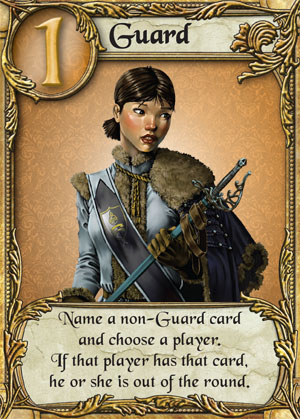
\includegraphics[scale=0.5]{Resources/Love_Letter_Card_Guard.png}
	\caption{Strażniczka} \label{fig:Love_Letter_Card_Guard}
\end{figure}
Na rysunku \ref{fig:Love_Letter_Card_Guard} przedstawiona jest karta typu Strażniczka. Zagrywając tę kartę należy wskazać jednego z pozostałych graczy i odgadnąć kartę którą posiada. Jeśli karta została prawidłowo odgadnięta, wskazany gracz odrzuca ją i przegrywa rundę.

\begin{figure}[h]
	\centering
	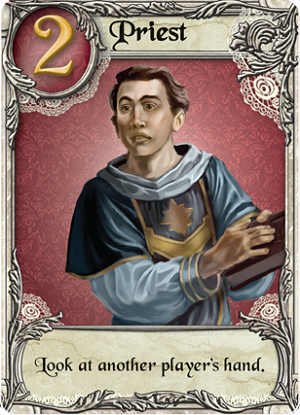
\includegraphics[scale=0.5]{Resources/Love_Letter_Card_Priest.png}
	\caption{Kapłan} \label{fig:Love_Letter_Card_Priest}
\end{figure}
Rysunek \ref{fig:Love_Letter_Card_Priest} przedstawia kartę typu Kapłan. Zagrywając tę kartę należy podglądnąć kartę wybranego gracza.

\clearpage
\begin{figure}[h]
	\centering
	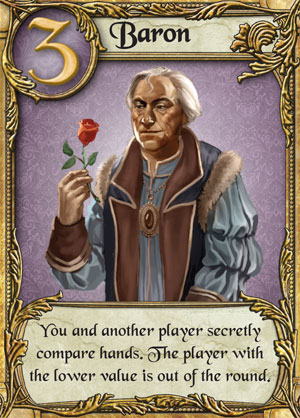
\includegraphics[scale=0.5]{Resources/Love_Letter_Card_Baron.png}
	\caption{Baron} \label{fig:Love_Letter_Card_Baron}
\end{figure}
Na rysunku \ref{fig:Love_Letter_Card_Baron} przedstawiona jest karta typu Baron. Po zagraniu tej karty należy w ukryciu porównać drugą posiadaną kartą z wybranym graczem. Następnie ten gracz, który ma kartę o mniejszej wartości odrzuca swoją kartę i przegrywa rundę. W przypadku remisu nic się nie dzieje.

\begin{figure}[h]
	\centering
	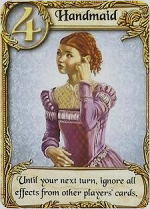
\includegraphics{Resources/Love_Letter_Card_Handmaid.png}
	\caption{Pokojówka} \label{fig:Love_Letter_Card_Handmaid}
\end{figure}
Rysunek \ref{fig:Love_Letter_Card_Handmaid} przedstawia kartę typu Pokojówka. Zagranie tej karty sprawia, że gracz jest niewrażliwy na efekt pozostałych kart do czasu swojej następnej tury.

\clearpage
\begin{figure}[h]
	\centering
	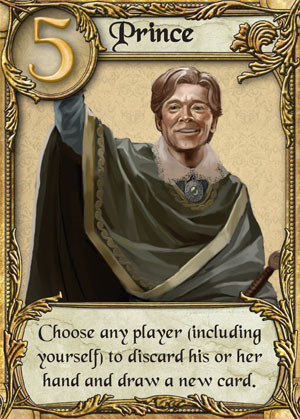
\includegraphics[scale=0.5]{Resources/Love_Letter_Card_Prince.png}
	\caption{Książe} \label{fig:Love_Letter_Card_Prince}
\end{figure}
Na rysunku \ref{fig:Love_Letter_Card_Prince} przedstawiona jest karta typu Książę. Zagranie pozwala wybrać dowolnego gracza (w tym siebie), zmusić go do odrzucenia posiadanej karty i pociągnięcia następnej.

\begin{figure}[h]
	\centering
	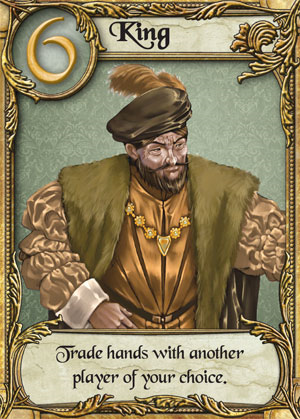
\includegraphics[scale=0.5]{Resources/Love_Letter_Card_King.png}
	\caption{Król} \label{fig:Love_Letter_Card_King}
\end{figure}
Rysunek \ref{fig:Love_Letter_Card_King} przedstawia kartę typu Król. Po jej zagraniu należy wymienić się drugą kartą z innym graczem.

\clearpage
\begin{figure}[h]
	\centering
	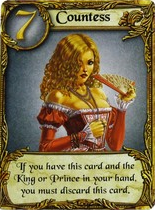
\includegraphics{Resources/Love_Letter_Card_Countess.png}
	\caption{Hrabina} \label{fig:Love_Letter_Card_Countess}
\end{figure}
Rysunek \ref{fig:Love_Letter_Card_Countess} przedstawia kartę typu Hrabina. Ta karta ma działanie pasywne. Nie wywiera efektu po zagraniu, natomiast zmusza gracza do jej zagrania jeśli równocześnie posiada na ręce kartę typu Książę lub Król.

\begin{figure}[h]
	\centering
	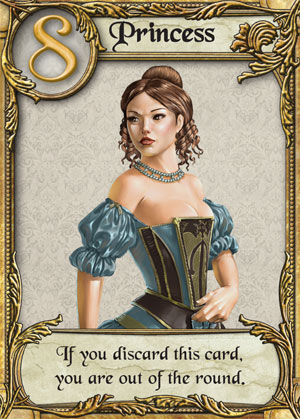
\includegraphics[scale=0.5]{Resources/Love_Letter_Card_Princess.png}
	\caption{Księżniczka} \label{fig:Love_Letter_Card_Princess}
\end{figure}
Na rysunku \ref{fig:Love_Letter_Card_Princess} przedstawiona jest karta typu Księżniczka. Zagranie tej karty oznacza natychmiastową przegraną w rundzie. Ta zasada działa również, gdy gracz został zmuszony do zagrania tej karty, np. przez efekt karty Książe.
\clearpage

\section{Analiza problemu}
\label{sec:opisProblemu}
Z wyżej przedstawionych zasad wynika, że gra cechuje się wysokim stopniem losowości i jest niedeterministyczna, więc można ją przedstawić jako problem optymalizacyjny$^{[\ref{bib:wiki_ProblemOptymalizacyjny}]}$. W związku z tym powstaje również pytanie, jaka jest najlepsza strategia mieszana bądź czysta$^{[\ref{bib:wiki_StrategiaTeoriaGier}]}$ maksymalizująca prawdopodobieństwo wygrania gry. Dla dalszych rozważań zakładam, że w gra toczy się pomiędzy dwoma graczami.

Najprostszym sposobem na znalezienie takiej strategii, byłoby stworzenie drzew probabilistycznych dla wszystkich możliwych stanów początkowych gry a następnie opracowanie algorytmu podejmowania decyzji opartego na danych statystycznych. Jednakże, ilość i rozmiar tych drzew może być zbyt duża by znaleźć rozwiązanie problemu w rozsądnym czasie. Z tego powodu postanowiłem najpierw oszacować ile jest wszystkich możliwych przebiegów gry. Nim przejdę do obliczeń, wprowadzę kilka definicji by ustandaryzować używane pojęcia:
\begin{itemize}
	\item \textit{Decyzja} - inaczej \textit{Zagranie}, jest to typ karty wraz ze sposobem jej wykorzystania. Przykładowo: Zagranie karty typu Strażniczka z wyborem karty typu Król, lub zagranie karty typu Książę z wyborem na gracza przeciwnego.
	\item \textit{Podjęcie decyzji} - to wybór zagrania według zastosowanego algorytmu, które zostanie użyte jako ruch w grze.
	\item \textit{Strategia} - ciąg decyzji podejmowanych według reguł określonych przez algorytm
	\item \textit{Scenariusz} - inaczej przebieg gry, chronologiczny ciąg decyzji podjętych przez obu graczy od początku do końca rundy; Jedna ze ścieżek w drzewie probabilistycznym dla danego stanu początkowego rundy, czyli pojedyncze rozwiązanie.
\end{itemize}

\subsection*{Oszacowanie ilości rozwiązań}
Na przebieg każdej rundy wpływ mają następujące czynniki:
\begin{itemize}
	\item Kolejność kart w talii na początku rundy
	\item Zagrywanie kart przez graczy
\end{itemize}
Zacząłem od oszacowania ilości możliwych rozwiązań. W każdej rundzie bierze udział wszystkie 16 kart. Zakładając, że każda z nich jest unikalna, to  liczba wszystkich możliwych kolejności kart to permutacja, którą obliczam wzorem podanym w [\ref{bib:tabliceMatematyczne}]:

\begin{center}
	$P_n = n!$ , gdzie $n\in N^+$
\end{center}

Dla  $n$ = 16, $n!=20 922 789 888 000$. Część kart się powtarza, więc tę liczbę należy jeszcze podzielić przez permutacje powtarzających się kart Strażniczki, Kapłana, Barona, Pokojówki oraz Księcia. Razem jest to $4! * 2! * 2! * 2! * 2! =  384$. Tak więc liczba unikalnych kolejności kart wynosi: 

\begin{center}
	$20 922 789 888 000 / 32 = 54486432000$ - 54mld, 864mln i 432 tys.
\end{center}

Należy zwrócić uwagę, że jest to górne oszacowanie. Może to się wydawać nieintuicyjne, bo przecież jeśli przetasujemy w zadany sposób talię to określimy tylko kolejność w jakiej gracze będą dociągać karty nie biorąc pod uwagę decyzji podjętych przez graczy, ale należy zauważyć, że te podjęte decyzje doprowadzą ewentualnie do innego stanu talii, który już został wzięty pod uwagę w obliczeniach. Co więcej, istnieją warunki zmniejszające zadane oszacowanie, ponieważ część kolejności kart może prowadzić do tego samego rozwiązania. Za przykład niech posłuży sytuacja, w której pierwszy gracz ma w ręce dwie karty typu Książę. O ile zagranie Księcia na przeciwnika nie skończy gry, to doprowadzi do zmiany układu talii na inny, który jest już wzięty pod uwagę w obliczeniach. W tym miejscu należałoby wskazać dolne oszacowanie, niemniej jednak te wyliczenia byłyby zbyt obszerne, a nie są głównym celem pracy.

Z uwagi na rząd wielkości, stworzenie optymalnej strategii na podstawie analizy statystycznej wszystkich dostępnych rozwiązań byłoby czasochłonne. Z tego powodu, zamiast odpowiadać na pytanie ,,Jaka jest najlepsza strategia podejmowania decyzji?'', dużo łatwiej będzie odpowiedzieć na pytanie ,,która z podanych strategii jest najlepsza?''. Kierując się tą zasadą, w następnym rozdziale opisałem wybrane strategie, których skuteczność sprawdzę implementując je w napisanej przeze mnie aplikacji. Pozostaje jeszcze sformalizować przedstawiony problem za pomocą modelu matematycznego.


\section{Opis formalny problemu}
W celu ujednolicenia używanych pojęć i skrótów, przedstawię je następująco:

\clearpage
\begin{table}[t]
	\caption{Pojęcia i skróty}
	\centering
	\begin{tabular}{|l|c|p{4cm}|c|}
		\hline
		\bf{Nazwa (typ) karty} & \bf{Skrót nazwy}  & \bf{Możliwe zagrania} & \bf{Skrót zagrania} \\ \hline
		Strażniczka & Str & Strażniczka z wyborem na [Nazwa karty] & Str\_Kap, Str\_Bar, ... , Str\_K-a  \\ \hline
		Kapłan & Kap & Zagranie kapłana & Kap\_Z \\ \hline
		Baron & Bar & Zagranie barona & Bar\_Z  \\ \hline
		Pokojówka & Pok & Zagranie pokojówki & Pok\_Z \\ \hline
		Książe & K-e & Książe na siebie; Książe na przeciwnika & K-e\_S, K-e\_P  \\ \hline
		Król & Krl & Zagranie Króla & Krl\_Z \\ \hline
		Hrabina & Hra & Zagranie Hrabiny & Hra\_Z \\ \hline
		Księżniczka & K-a & Zagranie Księżniczki & K-a\_Z \\ \hline
	\end{tabular}
\end{table}
Inne:
\begin{itemize}
	\item ,,ręka'' - karty, które gracz aktualnie posiada.
	\item $Z$ - zbiór zagrań (decyzji), oznaczanych jako $z$. Jest to zbiór wszystkich dostępnych decyzji w grze.
	\item $Z_i$ - zbiór zagrań (decyzji) dostępnych w danym stanie(węźle) $i$
	\item $DK$ - druga karta, którą gracz posiada w ręce.
	\item \textit{Typ Karty} - jeden z ośmiu rodzajów kart.
	\item $W(Karta)$ - wartość karty od 1 do 8.
\end{itemize}

Patrząc z perspektywy jednego z graczy, cała gra składa się z szeregu etapów (tur), gdzie w każdym etapie gracz podejmuje decyzje, a stan początkowy następnego etapu jest wynikiem dwóch akcji: podjętej decyzji (której efekt możemy przewidzieć z pewnym prawdopodobieństwem) i reakcji gracza drugiego, której prawdopodobieństwo jest nieokreślone. Dodatkowo, rzeczywisty stan każdego etapu nie jest w pełni znany graczowi. Z tych cech wynika, że grę ,,Love Letter'' możemy sklasyfikować jako \textbf{dynamiczny(wieloetapowy) proces podejmowania decyzji w warunkach niepewności}$^{[\ref{bib:matematyczneModeleKonfliktu_klasyfikacja}]}$. Jej zapis formalny można przedstawić jako grę w postaci ekstensywnej$^{[\ref{bib:matematyczneModeleKonfliktu_graEkstensywna}]}$:
\begin{center}
	$T = (S,R)$, gdzie
	\begin{itemize}
		\item $T$ - graf skierowany
		\item $S$ - zbiór wierzchołków (węzłów)
		\item $R$ - relacja określona na parach wierzchołków (łuki)
	\end{itemize}
\end{center}

Przypisując każdemu wierzchołkowi $s \in S$ jeden ze stanów rundy, a każdemu łukowi $r \in R$ decyzję danego gracza ze zbioru $Z$ lub udział losu, otrzymamy zapis pozwalający jednoznacznie określić możliwe przebiegi konkretnej gry, podjęte przez graczy decyzje, ich stan wiedzy na każdym etapie oraz wypłaty graczy (wynik gry).

Ponieważ w każdej rundzie bierze udział dwóch graczy, oznaczmy ich jako $P_1$ i $P_2$. Dodatkowo, część w której losowana jest karta oznaczmy jako $Los$. Zauważmy, że skoro korzeń $s_0$ to stan początkowy rundy przed losowaniem kart z talii, to wszystkie łuki wychodzące z $s_0$ są efektem losowania, a łuki z następnych poziomów należą kolejno do gracza $P_1$, $Losu$, gracza $P_2$ itd. Poglądowo zilustrowałem to w następujący sposób (Rys. \ref{fig:drzewo}):

\begin{figure}[h]
	\centering
	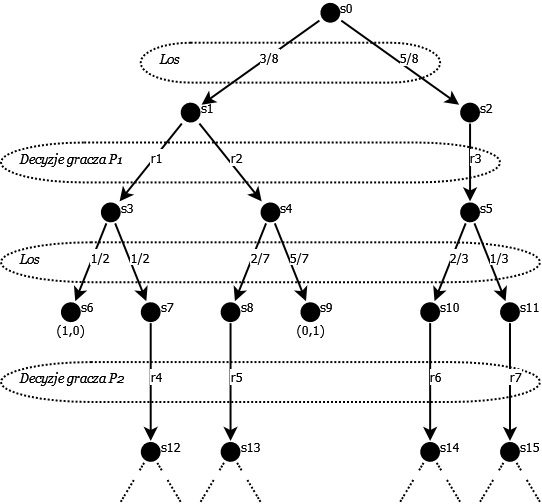
\includegraphics[scale=0.5]{Resources/drzewo2.png}
	\caption{Przykład drzewa gry w postaci ekstensywnej} 
	\label{fig:drzewo}
\end{figure}
Ogólne wnioski:
\begin{itemize}
	\item wszystkie łuki wychodzące z węzłów należących do $Losu$ oznaczone są prawdopodobieństwem sumującym się do 1.
	\item węzły $s_6$ i $s_9$ są liśćmi drzewa i zawierają wypłaty graczy (wynik gry) - 1 oznacza zwycięstwo, 0 oznacza przegraną. Przykładowo, w prezentowanym drzewie, w węźle $s_6$ wygrał gracz $P_1$.
	\item należy zauważyć, że węzły $r$ są ponumerowane i nie są wzajemnie jednoznaczne z zagraniami ze zbioru $Z$. Jak najbardziej wiele różnych węzłów może oznaczać to samo zagranie.
\end{itemize}

Zdarza się, że gracze nie wiedzą w jakim węźle danego poziomu drzewa się znajdują. Wracając do powyższego przykładu (Rys. \ref{fig:drzewo}) załóżmy, że łuki $r_4$ i $r_5$ są takim samym zagraniem dostępnym dla gracza $P_2$. Gracz nie wie czy gra znajduje się w stanie $s_7$ czy $s_8$, ponieważ oba stany udostępniają ten sam zbiór zagrań, co odzwierciedla niepełną wiedzę gracza $P_2$. Grupa takich stanów, które udostępniają ten sam zbiór zagrań, tworzy \textbf{zbiór informacyjny}. W dalszej części pracy takie zbiory będziemy określać jako $I_n$, a zbiór udostępnianych zagrań jako $X_n$ (zauważmy, że $X_n \subset Z$), gdzie $n$ oznacza poziom drzewa. Zbiór węzłów, które następują po węzłach z $I_n$ nazywamy \textbf{loterią}.

Przedstawiony model jednoznacznie określa stan gry i graczy. Dla uwzględnienia decyzyjności, do takiego modelu należy dodać jeszcze funkcję wyboru (decyzji). Oznaczmy ją jako $d$:
\begin{center}
	$d(s) \rightarrow r$, gdzie $r$ jest dowolnym łukiem wychodzącym ze stanu $s$
\end{center}

Jest to deklaracja ogólna. Zdecydowanie ważniejsze są funkcje wyboru należące do graczy $P_1$ i $P_2$, które uwzględniają zbiór informacyjny. Oznaczmy je odpowiednio jako $d_1$ i $d_2$. Ich postać będzie następująca:

\begin{center}
	$d_i(I_n, X_n) \rightarrow z$, gdzie $z$ jest dowolnym zagraniem należącym do $X_n$ i $i = \{1, 2\}$
\end{center}
W takiej postaci widać, że gracze podejmą decyzję mając niepełną informację na temat stanu gry. W następnym rozdziale przedstawiam algorytmy, które będą dokładnie definiować funkcję wyboru gracza.
